% this file is called up by thesis.tex
% content in this file will be fed into the main document
\chapter{Código/Manuales/Publicaciones}
\section{Código pantalla táctil}
\begin{verbatim}

/////////////////////////////////////
//programa para control de alto voltaje
//mediante la implementacion de LCD TOUCH TFT de 3.2
//
//
//
/////////////////////////////////////
#include <UTFT.h>
#include <URTouch.h>



//indicamos pines para hardware
UTFT    myGLCD(ILI9341_16,38,39,40,41);
URTouch  myTouch( 6, 5, 4, 3, 2);


//Definimos fuentes que utilizaremos
extern uint8_t SmallFont[];
extern uint8_t BigFont[];
extern uint8_t SevenSegNumFont[];

//variables que estaremos utilizando
int x,y,pantalla=1,k,voltaje=1,p=0,p1=0,p2=0,p3=0,vout=0;
char dato[20];

//variables para tomar datos de UART

String str = "";
const char separator = ',';
const int dataLength = 2;
int data[dataLength];
char vin[20];
      char current[20];


void botones1(){ ///////////////////////////////////////botones pantalla 1
  myGLCD.setFont(BigFont); 

  for (x=0; x<3; x++)
  {
    myGLCD.setColor(0, 0, 255);
    myGLCD.fillRoundRect (200, 10+(x*55), 310, 60+(x*55));
    myGLCD.setColor(255, 255, 255);
    myGLCD.drawRoundRect (200, 10+(x*55), 310, 60+(x*55));
    
  }

for (x=0; x<2; x++)
  {
    myGLCD.setColor(0, 0, 255);
    myGLCD.fillRoundRect (10+(x*155), 175, 155+(x*155), 225);
    myGLCD.setColor(255, 255, 255);
    myGLCD.drawRoundRect (10+(x*155), 175, 155+(x*155), 225);
    
  }



  
  myGLCD.setBackColor(0, 0, 255);
  myGLCD.print("ON 2", 220 , 30);
  myGLCD.print("ON 3", 220 , 85);
  myGLCD.print("ON 1", 220 , 140);
  //myGLCD.print("UART ON", 185 , 195);
  myGLCD.print("V SET", 40 , 190);
  myGLCD.print("CONFIG", 190 , 190);
  
  
  
  }
  
  
  
void marco1(int x1, int y1, int x2, int y2){ //////////////////////////marcos pantalla 1
  myGLCD.setColor(255, 0, 0);
  myGLCD.drawRoundRect (x1, y1, x2, y2);
  while (myTouch.dataAvailable())
  myTouch.read();
  myGLCD.setColor(255, 255, 255);
  myGLCD.drawRoundRect (x1, y1, x2, y2);
  
}

void touch1(){ ///////////////////////////////////////////////////////funciones de touch pantalla 1
  
      myTouch.read();
      x=myTouch.getX();
      y=myTouch.getY();

      if((x>=200) && (x<=310))
      {
        if((y>=10) && (y<=60)){ //boton ON 2
          marco1(200,10,310,60);
        }
        
        if((y>=65) && (y<=115)){ //boton ON 3
          marco1(200,65,310,115);

        }

        if((y>=120) && (y<=170)){ //boton ON 1
          marco1(200,120,310,170);
   
        }

       
      }

      if((y>=175) && (y<=225))
      {
        if((x>=10) && (x<=155)){ //boton V SET
          marco1(10,175,155,225);
          pantalla =2;
        }
      
        if((x>=165) && (x<=310)){ //boton config
          marco1(165,175,310,225);
          
        }
}
}

////////////////////////////// fin de pantalla 1


//////////////////////////////////////////////////////////////////////////// pantalla 2

void botones2(){ /////////////////////////////////////////////////////////// botones pantalla 2
  myGLCD.setBackColor(0,0,255);
  for (x=0; x<4; x++) //botones +
  {
    myGLCD.setColor(0, 0, 255);
    myGLCD.fillRoundRect (10+(x*60), 10, 60+(x*60), 60);
    myGLCD.setColor(255, 255, 255);
    myGLCD.drawRoundRect (10+(x*60), 10, 60+(x*60), 60);
    myGLCD.print("+", 27+(x*60), 27);
  }


  for (x=0; x<4; x++) //botones -
  {
    myGLCD.setColor(0, 0, 255);
    myGLCD.fillRoundRect (10+(x*60), 170, 60+(x*60), 220);
    myGLCD.setColor(255, 255, 255);
    myGLCD.drawRoundRect (10+(x*60), 170, 60+(x*60), 220);
    myGLCD.print("-", 27+(x*60), 190);
  }

  for (x=0; x<4; x++) //blanco 
  {
    myGLCD.setColor(255, 255, 255);
    myGLCD.fillRoundRect (10+(x*60), 70, 60+(x*60), 160);
    myGLCD.setColor(255, 0, 0);
    myGLCD.drawRoundRect (10+(x*60), 70, 60+(x*60), 160);
  //  myGLCD.print(p, 27+(x*60), 170);
  }

  myGLCD.setColor(0, 0, 255); /// boton set
   myGLCD.fillRoundRect(250,70,310,160);
   myGLCD.setColor(255, 255, 255);
   myGLCD.drawRoundRect(250,70,310,160);
   myGLCD.print("set" , 255,105);
  }

  void suma(int x1,int x2,int x3,int x4, int k, int w){ ///////////////////////algoritmo subir o bajar voltaje seteado
          myGLCD.setFont(SevenSegNumFont);
          myGLCD.setColor(0, 0, 0);
          myGLCD.setBackColor(255,255,255);
          int q;  
          if(x1 == 1){      //////////////////////////////////algoritmo kilos
            if(w==0 && p<9){
            vout=vout+1000;
            p=p+1;
            q=p*x1+p1*x2+p2*x3+p3*x4;
            sprintf(dato,"%d",q);
            }
            if(w==1 && p>0){
            vout=vout-1000;
            p=p-1;
            q=p*x1+p1*x2+p2*x3+p3*x4;
            sprintf(dato,"%d",q);
              
              }
            myGLCD.print(dato,20*x1+80*x2+140*x3+200*x4,90);
//            Serial.println(vout);
          }
          if(x2 == 1){ /////////////////////////////////////////algoritmo centena
            if(w==0 && p1<9){
            vout=vout+100;
            p1=p1+1;
            q=p*x1+p1*x2+p2*x3+p3*x4;
            sprintf(dato,"%d",q);
            }
            if(w==1 && p1>0){
            vout=vout-100;
            p1=p1-1;
            q=p*x1+p1*x2+p2*x3+p3*x4;
            sprintf(dato,"%d",q);
              
              }
            myGLCD.print(dato,20*x1+80*x2+140*x3+200*x4,90);
//            Serial.println(vout);
          }
          if(x3 == 1){ //////////////////////////////////////////algoritmo decenas
            if(w==0 && p2<9){
            vout=vout+10;
            p2=p2+1;
            q=p*x1+p1*x2+p2*x3+p3*x4;
            sprintf(dato,"%d",q);
            }
            if(w==1 && p2>0){
            vout=vout-10;
            p2=p2-1;
            q=p*x1+p1*x2+p2*x3+p3*x4;
            sprintf(dato,"%d",q);
              
              }
            myGLCD.print(dato,20*x1+80*x2+140*x3+200*x4,90);
            //Serial.println(vout);
          }
          if(x4 == 1){ ////////////////////////////////algoritmo unidades
            if(w==0 && p3<9){
            vout=vout+1;
            p3=p3+1;
            q=p*x1+p1*x2+p2*x3+p3*x4;
            sprintf(dato,"%d",q);
            }
            if(w==1 && p3>0){
            vout=vout-1;
            p3=p3-1;
            q=p*x1+p1*x2+p2*x3+p3*x4;
            sprintf(dato,"%d",q);
              
              }
            myGLCD.print(dato,20*x1+80*x2+140*x3+200*x4,90);
//            Serial.println(vout);
          }
          
           if(k==1){
            for(x=0 ; x<4 ; x++){
              sprintf(dato,"%d",p);
              myGLCD.print(dato,20,90);
              sprintf(dato,"%d",p1);
              myGLCD.print(dato,80,90);
              sprintf(dato,"%d",p2);
              myGLCD.print(dato,140,90);
              sprintf(dato,"%d",p3);
              myGLCD.print(dato,200,90);
              
              
              }
            
            }
    
    }
  
   void touch2(){ ////////////////////////////////////////////////////////touch pantalla 2
    myTouch.read();
      x=myTouch.getX();
      y=myTouch.getY();

      if((y>=10) && (y<=60)){ /////////////botones +
        if((x>=10) && (x<=60)){ //boton + kilos
          marco1(10,10,60,60);
          
          myGLCD.setFont(SevenSegNumFont); 
          suma(1,0,0,0,0,0);
         
          
        }

        if((x>=70) && (x<=120)){ //boton + centena
          marco1(70,10,120,60);
          suma(0,1,0,0,0,0);
          
          
        }

        if((x>=130) && (x<=180)){ //boton + decena
          marco1(130,10,180,60); 
          suma(0,0,1,0,0,0);
          
        }

        if((x>=190) && (x<=240)){ //boton + unidad
          marco1(190,10,240,60);
          suma(0,0,0,1,0,0);
          
        }
        }


        if((y>=170) && (y<=220)){ ////////////botones -
          
        if((x>=10) && (x<=60)){ //boton + kilos
          marco1(10,170,60,220);
          suma(1,0,0,0,0,1);
        }

        if((x>=70) && (x<=120)){ //boton + centena
          marco1(70,170,120,220);
          suma(0,1,0,0,0,1);
        }

        if((x>=130) && (x<=180)){ //boton + decena
          marco1(130,170,180,220);
          suma(0,0,1,0,0,1);
        }

        if((x>=190) && (x<=240)){ //boton + unidad
          marco1(190,170,240,220);
          suma(0,0,0,1,0,1);
        }
        }

        if((x>=250) && (x<=310)){ // boton SET

          if((y>=70) && (y<=160)){
            marco1(250,70,310,160);
            pantalla =1;
            if(vout >=0 && vout <=1000){
            Serial.println(vout);
            }
            }
          

        }
       
    
    }


///////////////////////fin pantalla set voltaje

void setup(){
  myGLCD.InitLCD();
  myGLCD.clrScr();
  myTouch.InitTouch();
  myTouch.setPrecision(PREC_HI);
  Serial.begin(9600);
  Serial.setTimeout(50);
  }
void vinput(){
  
      str = Serial.readStringUntil('\n');
      for (int i = 0; i < dataLength ; i++)
      {
         int index = str.indexOf(separator);
         data[i] = str.substring(0, index).toInt();
         str = str.substring(index + 1);
      }
      
      for (int i = 0; i < sizeof(data) / sizeof(data[0]); i++)    
      {
        Serial.print(data[i]); 
      Serial.print('\t');} 
      Serial.println();
      
                  myGLCD.setFont(BigFont);
                  sprintf(vin, "%d",data[0]);
                  sprintf(current, "%d", data[1]);
                  myGLCD.print("     " ,10,50);
                  myGLCD.print("     " ,10,70);
                  myGLCD.setBackColor(0,0,0);
                  myGLCD.setColor(255,255,255);
                  myGLCD.print(vin ,10,50);
                  myGLCD.print(current ,10,70);
  }
void loop(){

////////////////////////////////////pantalla 1
if(pantalla == 1){
    myGLCD.fillScr(VGA_BLACK);
    botones1();
    myGLCD.setFont(BigFont); 
    char set[25];
    sprintf(set, "%d",vout);
    myGLCD.setBackColor(0,0,0);
    myGLCD.print(set ,10,100);
    myGLCD.print("V set" ,100,100);
    myGLCD.print("V out" ,100,50);
    myGLCD.print("mA out" ,100,70);
    myGLCD.print(vin ,10,50);
    myGLCD.print(current ,10,70);
    while(true)
         {
          if(myTouch.dataAvailable())touch1();
          if(pantalla == 2 )break;

      if (Serial.available()>0){vinput();}
   
   
            }
            }
          
        
//////////////////////////////////pantalla 2
if(pantalla == 2){
  myGLCD.fillScr(VGA_BLACK);
  
  botones2();
  
  suma(0,0,0,0,1,0);
  while(true)
    {
      if(myTouch.dataAvailable())touch2();
      if(pantalla == 1)break;
    }
  }


  }

\end{verbatim}

\section{Diagrama electrónico IBT-2}
\begin{figure}[H]
\centering
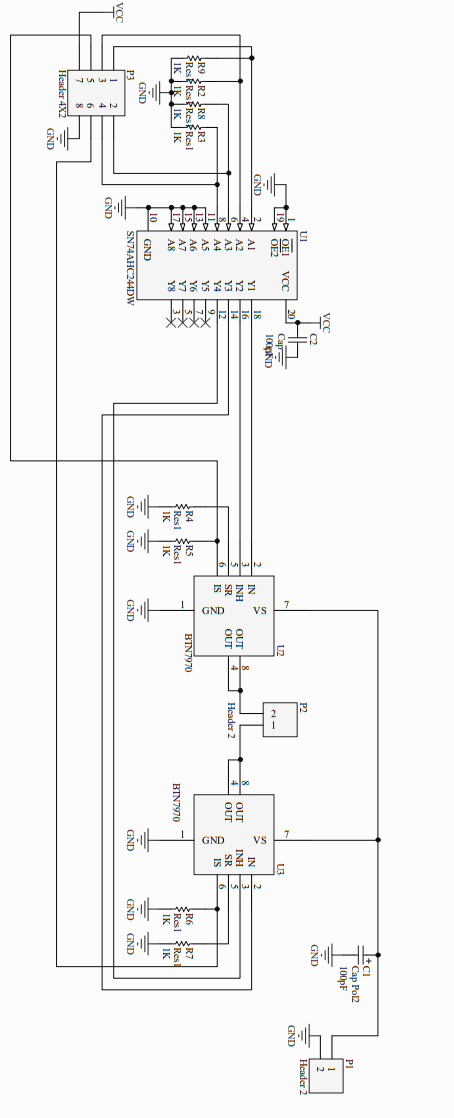
\includegraphics[width=6cm]{Capitulo3/figs/ibt2.png}
\caption{diagrama puente H}
\end{figure}